\documentclass[a4paper,12pt]{article}

%%%%%%%%%%%%%%%%%%%%%%%%%%%%%%%%%%%%%%%%%%%%%%%%
% Packages
%%%%%%%%%%%%%%%%%%%%%%%%%%%%%%%%%%%%%%%%%%%%%%%%

\usepackage[right=2.5cm, left=2.5cm, top=2.5cm, bottom=2.5cm]{geometry} 
\usepackage[portuguese]{babel}
\usepackage[T1]{fontenc}
\usepackage[utf8]{inputenc}
\usepackage{enumerate}

% no indentation
%\usepackage{setspace}
%\setlength{\parindent}{0in}

\usepackage{graphicx} 
\usepackage{float}
\usepackage{xcolor}
\usepackage{tikz}
\usetikzlibrary{positioning}

\usepackage{url}
\usepackage{hyperref}

\usepackage{mathtools}
\usepackage{amssymb, amsthm}

% headers
\usepackage{fancyhdr}

%%%%%%%%%%%%%%%%%%%%%%%%%%%%%%%%%%%%%%%%%%%%%%%%
% Proper definitions
%%%%%%%%%%%%%%%%%%%%%%%%%%%%%%%%%%%%%%%%%%%%%%%%

\newcommand{\R}{\mathbb{R}}
\newcommand{\Q}{\mathbb{Q}}
\newcommand{\Z}{\mathbb{Z}}
\newcommand{\tr}{\operatorname{tr}}
\newcommand\eq{\mathrel{\overset{\makebox[0pt]{\mbox{\normalfont\tiny\sffamily def}}}{=}}}

\newtheoremstyle{exer}{}{}{\color{blue}}{}{\color{blue}\bfseries}{}{ }{}

\newtheorem*{aff}{Afirmação}

\theoremstyle{exer}
\newtheorem{exercise}{Exercício}

\theoremstyle{definition}

\newcommand{\enu}[1]{\textcolor{blue}{#1}}

%%%%%%%%%%%%%%%%%%%%%%%%%%%%%%%%%%%%%%%%%%%%%%%%
% Header (and Footer)
%%%%%%%%%%%%%%%%%%%%%%%%%%%%%%%%%%%%%%%%%%%%%%%%

\pagestyle{fancy} 
\fancyhf{}

\lhead{\footnotesize EDP: Lista 1}
\rhead{\footnotesize Prof. Moacyr} 
\cfoot{\footnotesize \thepage} 


\begin{document}

%%%%%%%%%%%%%%%%%%%%%%%%%%%%%%%%%%%%%%%%%%%%%%%%
% Title section of the document
%%%%%%%%%%%%%%%%%%%%%%%%%%%%%%%%%%%%%%%%%%%%%%%%

\thispagestyle{empty} 

\begin{tabular*}{0.95\textwidth}{l @{\extracolsep{\fill}} r} 
    {\large \bf Equações Diferenciais Parciais 2021.2} &  \\
    Escola de Matemática Aplicada, Fundação Getulio Vargas &  \\
    Professor Moacyr Alvim Horta Barbosa da Silva &  \\ 
    Monitor Lucas Machado Moschen & Entrega 23/08/2021\\
    \hline \\
\end{tabular*}
\vspace*{0.3cm} 

\begin{center}
	{\Large \bf Lista 1} 
	\vspace{2mm}
	%{\bf Lucas Machado Moschen}	
\end{center}  
\vspace{0.4cm}

\begin{exercise}
    Indique quais das equações abaixo são lineares
    \begin{enumerate}[(a)]
        \item $y^my'' + (y')^{2m} = t^2y^2$
        \item $y'' + ty' + t^2y = t^3$
        \item $y''y' + y^4 - ty = t^2$ 
        \item $y' + \sin(t)y = 0$
    \end{enumerate}
\end{exercise}

Por definição, uma equação linear diferencial é um polinômio linear na função
desconhecida (no caso $y$) e nas suas derivadas por conseguinte. Ela tem a
forma:
\begin{equation}
    \label{eq:linear-edo}
    a_0(t)y + a_1(t)\frac{\partial y}{\partial t} + a_2(t)\frac{\partial^2 y}{\partial t^2} + \dots + a_n(t)\frac{\partial^n y}{\partial t^n} + b(t) = 0, 
\end{equation}
em que $a_i(\cdot), i = 1,\dots, n$ e $b(\cdot)$ são funções arbitrárias
diferenciáveis. Por esse motivo, observe que a letra (a) e (c) são altamente
não lineares devido ao termos de grau maior que 1 $y^m$ e $y^4$,
respectivamente. Já as letras (b) e (d) são bem comportadas como descrito
acima \eqref{eq:linear-edo}.

\begin{exercise}
    Exiba duas soluções do problema de valor inicial $y'=y^{2/3}$ com $y(0) =
    0$. Mostre que se $f:\R \to \R$ for diferenciável com derivada contínua,
    então o problema de valor inicial $y' = f(y)$ com $y(0) = y_0$ tem uma única solução na vizinhança de $y_0$.
\end{exercise}

A ideia é observar que $f(y) = y^{2/3}$ são é diferenciável na origem. De fato
$f'(y) = \frac{2}{3}y^{-1/3}$ que não é definido quando $y = 0$. Desta forma,
o teorema da existência é garantido, pela continuidade de $f$, mas não não
vale a unicidade das soluções. Por isso, faz sentido procurar mais de uma
solução. Para resolver:

\begin{enumerate}
    \item Primeiro observe que se $y(t) = 0$, para todo $t$, teremos que 
    $$
    y'(t) = 0 = 0^{2/3} = y(t)^{2/3}, 
    $$
    para todo $t$. Assim a solução identicamente nula é válida.
    
    \item Usemos a ideia de variáveis separáveis que estudamos em cálculo: 
    $$
    \frac{y'}{y^{2/3}} = 1 \implies \int \frac{y'}{y^{2/3}}\, dy  = t + C, 
    $$
    em que $C$ é uma constante. Assim, 
    $$
    3y^{1/3}(t) = t + C \implies y(t) = \left(\frac{t}{3} + K\right)^3, 
    $$
    mas $K = 0$, pois $y(0) = K^3 = 0$. Assim $y(t) = \dfrac{t^3}{27}$ também é
   solução. 
    
\end{enumerate}

{\bf Prova de existência e unicidade}

Considere o sistema autônomo $y' = f(y)$ com condição inicial $y(0) = y_0$ e
$f : \R \to \R$ diferenciável com derivada contínua. Nesse caso, se provarmos
que $f$ é
uniformemente Lipschitz contínua em $y$, vale o teorema de Picard-Lindelöf.
Seja $[y_0-\epsilon, y_0 + \epsilon]$ um intervalo fechado com $\epsilon > 0$. Como a
derivada de $f$ é contínua, então pelo Teorema de Weierstrass, ela assume seu
máximo e mínimo em pontos $y_1$ e $y_2$ so intervalo. Seja 
$$
M = f'(y_1), m = f'(y_2)
$$
os valores máximo e mínimo respectivamente e seja $K = \max(|m|, |M|)$. Assim,
pelo Teorema do Valor Médio, sejam $x_1, x_2$ dois pontos do intervalo, existe
$z \in (x_1, x_2)$ tal que, 
$$
|f(x_1) - f(x_2)| = |f'(z)||(x_1 - x_2)| \le K|x_1 - x_2|,  
$$
o que mostra a condição de Lipschitz. 

\begin{exercise}
    Encontre a solução geral das equações abaixo. Depois use um software para
    desenhar curvas das soluções com vários valores iniciais. Você pode usar o
    Dfield disponível em \url{http://math.rice.edu/~dfield/dfpp.html} 
\end{exercise}

\begin{enumerate}[{\color{blue} a)}]
    \item \enu{$y' - 2y = 4 - t$.}
    
    Considere o fator de integração: $I(t) = e^{\int_0^t (-2)ds} = e^{-2t}$.
    Assim, temos que a solução geral pode ser expressa por 
    $$y(t) = I(t)^{-1}\int I(t)(4 - t)dt,$$
    isto é:
    \begin{equation}
        \begin{split}
            y(t) &= e^{2t}\int e^{-2t}(4 - t)dt \\
            &= e^{2t}[4\int e^{-2t}dt - \int te^{-2t}dt] \\
            &= e^{2t}\left[-2e^{-2t} - \left(\frac{-1}{2}te^{-2t} + \int \frac{1}{2}e^{-2t}\right)\right]dt \\
            &= e^{2t}\left[-2e^{-2t} + \frac{1}{2}te^{-2t} + \frac{1}{4}e^{-2t} + c\right], c \in \mathbb{R} \\
            &= -\frac{7}{4} + \frac{1}{2}t + ce^{2t}
        \end{split}
    \end{equation}

    Concluo que $y(t) = -\frac{7}{4} + \frac{1}{2}t + ce^{2t}$. Se $y(0) = y_0$, temos que $y_0 = -\frac{7}{4} + c \implies c = y_0 + \frac{7}{4}$.

    \item \enu{$ty' + y = 3t \cdot \cos(2t), t > 0$.} 
    
    Usando a regra do produto para derivação, podemos reescrever o problema
    para  
    $$ty' + y = (ty)' = 3t\cdot \cos(2t).$$ 
    Assim, temos que:
    \begin{equation}
        \begin{split}
            ty &= \int 3t\cdot \cos(2t) dt \\
            &= \frac{3t}{2}\sin(2t) - \int \frac{3}{2}\sin(2t)dt \\
            &= \frac{3t}{2}\sin(2t) + \frac{3}{4}\cos(2t) + c, c \in \mathbb{R}
        \end{split}
    \end{equation}

    Como $t \neq 0$, concluo que $y(t) = \frac{3}{2}\sin(2t) + \frac{3}{4t}\cos(2t) + \frac{c}{t}, c \in \mathbb{R}$.  Se $y(\pi) = y_0$, temos que $y_0 = \frac{3}{4\pi} + \frac{c}{\pi} \implies c = y_0\pi - \frac{3}{4}$ 


    \item \enu{$y' +2ty = 2te^{-t^2}$. }
    
    Considere o fator de integração: $I(t) = e^{\int_0^t (2s)ds} = e^{t^2}$. Como fizemos em a, 

    \begin{align}
    y(t) = e^{-t^2} \int e^{t^2}(2te^{-t^2})dt = e^{-t^2} \int 2t dt = e^{-t^2}[t^2 + c] = ce^{-t^2} + t^2e^{-t^2}, c \in \mathbb{R}
    \end{align}

    Concluo que a solução geral é $ce^{-t^2} + t^2e^{-t^2}$. Se $y(0) = y_0$, temos que $y_0 = c$

\end{enumerate}

\begin{figure}
    \centering
    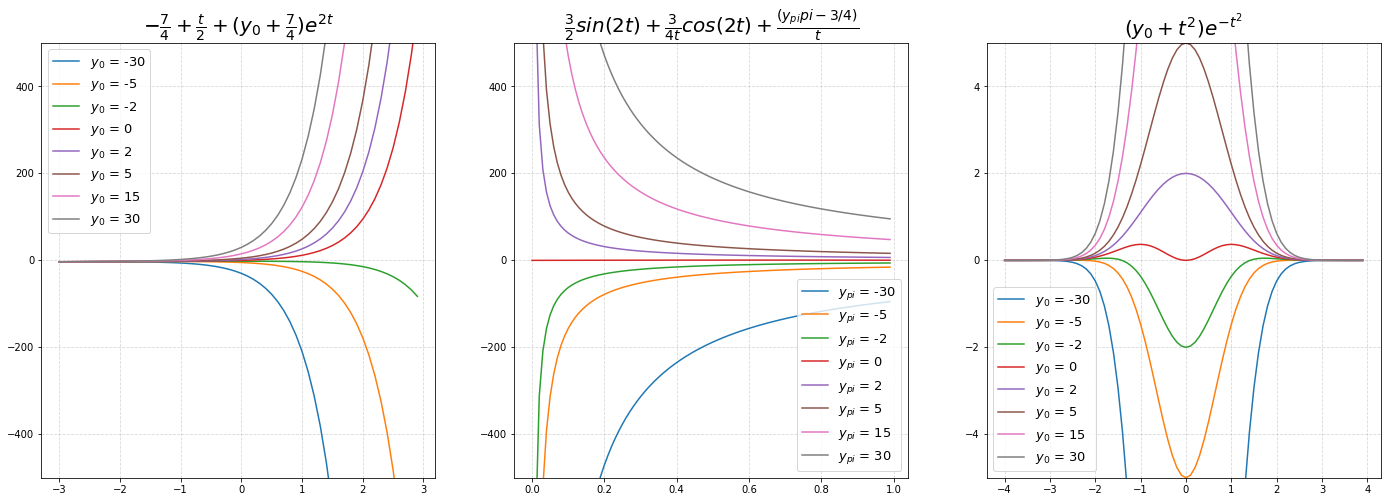
\includegraphics[width=\textwidth]{images/exercise2.png}
    \caption{Usando Matplotlib, observe como diferentes soluções podem alterar a direção das soluções.}
\end{figure}

\begin{exercise}
    Mostre que qualquer combinação afim de soluções particulares de uma
    equação diferencial linear $E$ também é solução de $E$. (Ou seja, o
    conjunto das soluções de equação diferencial linear é uma variedade afim).
\end{exercise}

Seja $E$ uma equação diferencial linear expressa da seguinte forma:
\begin{equation}
    \label{eq:E}
    \sum_{i= 0}^m a_i(x)y^{(i)} + b(x) = 0.
\end{equation}

Vou provar a afirmação por indução no número de soluções particulares $n$.
Sejam $y_1$ e $y_2$ soluções particulares de \eqref{eq:E}. Tome
$\alpha \in \mathbb{R}$. Vou provar que 
$$\alpha y_1 + (1 - \alpha)y_2 = y_2 + \alpha(y_1 - y_2)$$ 
também é solução de \eqref{eq:E}. Usando a linearidade da derivada: 

\begin{equation}
    \begin{split}
        \sum_{i = 0}^m a_i(x)&[\alpha y_1 + (1 - \alpha)y_2]^{(i)} + b(x) \\
        &= \sum_{i = 0}^m a_i(x)[\alpha y_1^{(i)} + (1 - \alpha)y_2^{(i)}] + b(x) \\
        &= \sum_{i = 0}^m a_i(x)\alpha y_1^{(i)} + a_i(x)(1 - \alpha)y_2^{(i)} + b(x) \\
        &= \alpha\sum_{i = 0}^m a_i(x)y_1^{(i)} + (1 - \alpha)\sum_{i = 0}^m a_i(x)y_2^{(i)} + b(x) \\
        &= \alpha\sum_{i = 0}^m a_i(x)y_1^{(i)} + (1 - \alpha)\sum_{i = 0}^m a_i(x)y_2^{(i)} + b(x) + \alpha b(x) - \alpha b(x) \\
        &= \alpha\left[\sum_{i = 0}^m a_i(x)y_1^{(i)} + b(x)\right] + (1 - \alpha)\left[\sum_{i = 0}^m a_i(x)y_2^{(i)} + b(x)\right] \\
        &= 0,  
\end{split}
\end{equation}
dado que ambas são soluções de \eqref{eq:E}. Concluo que $\alpha y_1 + (1 -
\alpha)y_2$ é solução para \eqref{eq:E}. 

Suponha a hipótese de indução, isto é, se $y_1, ..., y_n$ são soluções
particulares de \eqref{eq:E}, então qualquer combinação afim delas é solução.
Considere, então, a solução $y_{n+1}$ particular para \eqref{eq:E}. Tome
$\alpha_1, ..., \alpha_{n+1} \in \mathbb{R}$, tal que $\sum_{i=1}^{n+1}
\alpha_i = 1$. Sabemos que $$y^* \overset{def}{=} \sum_{i=1}^{n} \frac{\alpha_i}{1 - \alpha_{n+1}}
y_i$$ 
é solução para a equação \eqref{eq:E} pela hipótese de indução, dado que 
$\sum_{i=1}^n \frac{\alpha_i}{1 - \alpha_{n+1}} = 1$. Portanto, como provamos no caso particular acima,  $(1 - \alpha_{n+1}) y^{*} + \alpha_{n+1}y_{n+1}$ é solução para \eqref{eq:E}, isto é: 
$$
(1 - \alpha_{n+1}) y^{*} + \alpha_{n+1}y_{n+1} = (1 - \alpha_{n+1})\sum_{i=1}^{n} \frac{\alpha_i}{1 - \alpha_{n+1}} y_i + \alpha_{n + 1}y_{n+1} = \sum_{i=1}^{n+1} \alpha_i y_i 
$$
é solução da equação \eqref{eq:E}. Provamos então, por indução, que qualquer combinação afim de soluções particulares é solução também, isto é, esse conjunto de soluções é uma variedade afim.

\begin{exercise}
    Considere a equação $16y'' - 8y' + 145y = 0$.  Descreva a equação diferencial de segunda
    ordem deste exercício na forma de um sistema de equações diferenciais de primeira ordem.
    Use um pacote computacional (\url{http://math.rice.edu/~dfield/pplane.html}, por exemplo) para
    traçar várias soluções. Encontre a solução exata para o problema de valor inicial com
    condições iniciais $y(0) = -2$ e $y'(0) = 1$. 
\end{exercise}

Defina a variável $x = y'$, tal que $x' = y'' = \frac{1}{16}(8y' - 145y)$.
Assim, a equação pode ser escrita como o sistema linear:

$$
\begin{cases} 
x' = \frac{1}{2}x - \frac{145}{16}y \\ 
y' = x. \\ 
\end{cases}
$$

Considere a forma matricial do sistema: 

$$
A = \begin{bmatrix} 1/2 & -145/16 \\ 1 & 0 \end{bmatrix}
$$

O polinômio característico dessa matriz é 
$$\lambda^2 - \frac{1}{2}\lambda + \frac{145}{16} = 0.$$ 
Assim, os autovalores de $A$ são $\frac{1}{4} \pm 3i$ e os autovetores correspondentes são $(1/4 + 3i, 1)$ e $(1/4 - 3i, 1)$  
Como os autovalores são valores complexos, a solução é uma combinação de senos
e cossenos. Considere a seguinte decomposição da matriz de $A$:

$$
A = \begin{bmatrix} 3 & 1/4 \\ 0 & 1 \end{bmatrix}\begin{bmatrix} 1/4 & -3 \\ 3 & 1/4 \end{bmatrix}\cdot 1/3\begin{bmatrix} 1 & -1/4 \\ 0 & 3 \end{bmatrix}\begin{bmatrix} x_0 \\ y_0 \end{bmatrix}
$$

Desta mentira podemos calcular a exponencial dessa matriz:

\begin{equation}
    \begin{split}
        \begin{bmatrix} x(t) \\ y(t) \end{bmatrix} &= \begin{bmatrix} 3 & 1/4 \\ 0 & 1 \end{bmatrix}e^{1/4t}\begin{bmatrix} \cos(3t) & -\sin(3t) \\ \sin(3t) & \cos(3t) \end{bmatrix}\cdot 1/3\begin{bmatrix} 1 & -1/4 \\ 0 & 3 \end{bmatrix}\begin{bmatrix} x_0 \\ y_0 \end{bmatrix}\\
        &= e^{1/4t}\begin{bmatrix} 3\cos(3t) + 1/4\sin(3t) & -3\sin(3t) + 1/4\cos(3t) \\ \sin(3t) & \cos(3t) \end{bmatrix}\begin{bmatrix} x_0/3 -1/12y_0 \\ y_0 \end{bmatrix} \\
        &= e^{1/4t} \begin{bmatrix} (x_0 - y_0/4 + y_0/4)\cos(3t) + (x_0/12 - y_0/48 - 3y_0)\sin(3t) \\ 
        (x_0/3 - y_0/12)\sin(3t) + y_0\cos(3t)\end{bmatrix} \\
        &= e^{1/4t} \begin{bmatrix} x_0\cos(3t) + (x_0/12 - 145y_0/48)\sin(3t) \\ 
        (x_0/3 - y_0/12)\sin(3t) + y_0\cos(3t)
        \end{bmatrix}
    \end{split}
\end{equation}

Agora vamos calcular para o caso em que $y(0) = -2$ e$ x(0) = y'(0) = 1$. Assim: 

$$
\begin{bmatrix} x(t) \\ y(t) \end{bmatrix} = e^{1/4t}\begin{bmatrix} \cos(3t) + (1/12 + 145/24)\sin(3t) \\ 
(1/3 + 1/6)\sin(3t) - 2\cos(3t) \end{bmatrix} = e^{1/4t}\begin{bmatrix} \cos(3t) + 49/8\sin(3t) \\ 
1/2\sin(3t) - 2\cos(3t) \end{bmatrix}
$$

Como estamos apenas preocupados com $y$, temos que: 

$$y(t) = e^{1/4t}\left[\frac{1}{2}\sin(3t) - 2\cos(3t)\right].$$

\begin{figure}[!hb]
    \centering
    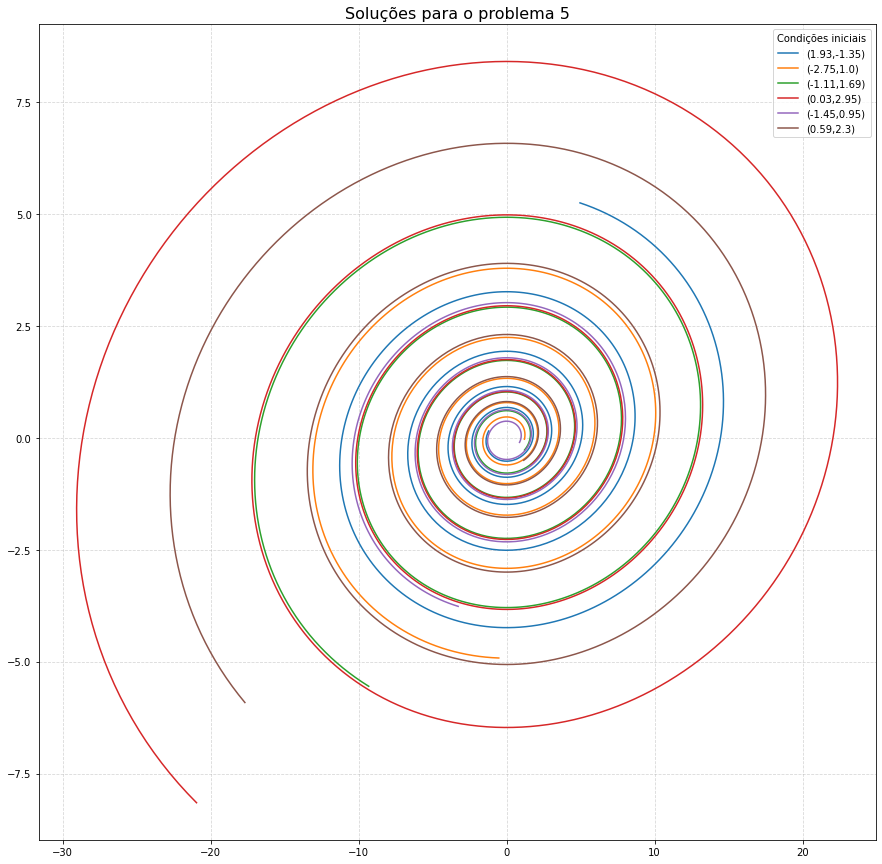
\includegraphics[width=0.7\textwidth]{images/exercise5.png}
    \caption{Usando Matplotlib, observe como diferentes soluções podem alterar a direção das soluções.}
\end{figure}

\end{document}